\section{Tutorial A14B}

\begin{problem}
    For each of the following situations, determine whether it can be modelled by a binomial distribution, geometric distribution, a Poisson distribution, or neither of the mentioned.
    \begin{enumerate}
        \item The number of heads obtained when a biased coin is tossed three times.
        \item The number of phone calls received in a randomly chosen hour.
        \item The number of accidents occurring in a factory in a randomly chosen week.
        \item The number of accidents until the first fatal accident at a traffic junction.
        \item The number of red balls obtained when 3 balls are chosen from a bag containing 4 red, 3 green and 3 white balls
        \begin{enumerate}
            \item with replacement;
            \item without replacement.
        \end{enumerate}
        \item The number of typing errors on a randomly chosen page in a draft of a novel.
        \item The number of seeds in a chosen packet of 12 seeds that fail to germinate.
        \item The number of throws of a die until a six is obtained.
    \end{enumerate}
\end{problem}
\begin{solution}
    \begin{table}[H]
        \centering
        \begin{tabular}{|l|c|}
        \hline
        \textbf{Part} & \textbf{Distribution} \\ \hline\hline
        (a) & Binomial \\ \hline
        (b) & Poisson \\ \hline
        (c) & Poisson \\ \hline
        (d) & Geometric \\ \hline
        (e)(i) & Binomial \\ \hline
        (e)(ii) &  - \\ \hline
        (f) & Poisson \\ \hline
        (g) & Binomial \\ \hline
        (h) & Geometric \\ \hline
        \end{tabular}
    \end{table}
\end{solution}

\begin{problem}
    Explain why each of the following situations is not a good model for the proposed distribution.
    \begin{enumerate}
        \item Using the Poisson distribution to model the number of cars sold at a particular car dealer in a randomly chosen year.
        \item Using the Binomial distribution to model the number of family members that will vote for Party A in the coming election.
        \item Using the Poisson distribution to model the number of people using a particular ATM during a randomly chosen day.
        \item Using the Geometric distribution to model the number of train trips for a particular train before the first breakdown.
    \end{enumerate}
\end{problem}
\begin{solution}
    \begin{ppart}
        Over the course of a year, the mean rate will likely not be uniform. For instance, the car dealer may only be open on weekdays, so the mean rate on weekdays is different from that on weekends.
    \end{ppart}
    \begin{ppart}
        The probability that one will vote for Party A is not uniform.
    \end{ppart}
    \begin{ppart}
        Over the course of a day, the mean rate will likely not be uniform. For instance, the mean rate at night will be less than the mean rate in the afternoon.
    \end{ppart}
    \begin{ppart}
        The trials are not independent. For instance, wear and tear from previous trials will affect the probability that the next train will break down.
    \end{ppart}
\end{solution}

\begin{problem}
    Calculate the probability that in a group of ten people,
    \begin{enumerate}
        \item none has his or her birthday on a Saturday,
        \item at least two have their birthdays on Saturday,
        \item more than two but at most five have their birthdays on Saturday.
        \item less than four have their birthdays on other days except Saturday,
    \end{enumerate}
    Find also the mean number of people whose birthday falls on Saturday.
\end{problem}
\begin{solution}
    Let $X$ be the number of people with a birthday on Saturday. Note that $X \sim \Binom{10}{1/7}$.
    \begin{ppart}
        $\P{X = 0} = 0.214$.
    \end{ppart}
    \begin{ppart}
        $\P{X \geq 2} = 1 - \P{X \leq 1} = 0.429$.
    \end{ppart}
    \begin{ppart}
        $\P{2 < X < \leq 5} = \P{X = 3} + \P{X = 4} + \P{X = 5} = 0.161$.
    \end{ppart}
    \begin{ppart}
        $\P{X > 6} = 1 - \P{X \leq 6} = 9.77 \times 10^{-5}$.
    \end{ppart}

    Since $n = 10$ and $p = 1/7$, the expected value of $X$ is \[\E{X} = np = \frac{10}{7}.\]
\end{solution}

\begin{problem}
    In a binomial experiment, the mean number of successful trials is 24 and the variance is 20. Find the number of trials conducted and the probability of success for each trial.
\end{problem}
\begin{solution}
    Let $n$ be the number of trials and $p$ be the probability of success of each trial. We have \[\m = np = 24 \quad \land \quad \s^2 = np(1-p) = 20.\] Thus, \[p = 1 - \frac{20}{np} = \frac16 \implies n = \frac{24}{p} = 144.\]
\end{solution}

\begin{problem}
    If $Y \sim \Po{2.5}$, state the expected value, $\m$, and the standard deviation, $\s$, of $Y$. Use your GC to evaluate the following correct to 3 significant figures.
    \begin{enumerate}
        \item $\P{Y = 3}$
        \item $\P{Y > 4.5}$
        \item $\P{Y \leq 5}$
        \item $\P{6 < Y < 10}$
        \item $\P{Y \text{ is 0 or 1}}$
        \item $\P{\abs{Y - \m} < \s}$
    \end{enumerate}
\end{problem}
\begin{solution}
    Since $Y$ follows a Poisson distribution, $\m = \s^2 = 2.5$, whence $\s = \sqrt{2.5}$.

    \begin{ppart}
        $\P{Y = 3} = 0.214$.
    \end{ppart}
    \begin{ppart}
        $\P{Y > 4.5} = 1- \P{Y \leq 4} = 0.109$.
    \end{ppart}
    \begin{ppart}
        $\P{Y \leq 5} = 0.958$.
    \end{ppart}
    \begin{ppart}
        $\P{6 < Y < 10} = \P{Y \leq 9} - \P{Y \leq 6} = 0.0139$.
    \end{ppart}
    \begin{ppart}
        $\P{Y \text{ is 0 or 1}} = \P{Y = 0} + \P{Y = 1} = 0.287$.
    \end{ppart}
    \begin{ppart}
        $\P{\abs{Y - \m} < \s} = \P{2.5 - \sqrt{2.5} < Y < 2.5 + \sqrt{2.5}} = \P{1 \leq Y \leq 4} = \P{Y \leq 4} - \P{Y = 0} = 0.809$.
    \end{ppart}
\end{solution}

\begin{problem}
    Epple Company manufactures many E-phones. It is known that 1\% of the E-phones manufactured are defective.
    \begin{enumerate}
        \item A random sample of $n$ phones was selected. Using an algebraic method, find the smallest value of $n$ such that the probability that there is at least one defective phone in the sample is more than 0.95.
        \item A carton, which consists of 24 E-phones, will be rejected if there are at least two defective phones. Show that the probability that a randomly chosen carton is being rejected is 0.0239.
    \end{enumerate}
\end{problem}
\begin{solution}
    \begin{ppart}
        Let $X$ be the number of defective phones in the sample. Then $X \sim \Binom{n}{0.01}$. Consider $\P{X \geq 1} \geq 0.95$: \[\P{X \geq 1} \geq 0.95 \implies \P{X = 0} = 0.99^n \leq 0.05 \implies n \geq 298.1.\] Since $n \in \NN$, the least $n$ is $299$.
    \end{ppart}
    \begin{ppart}
        Take $n = 24$. Then \[\P{X \geq 2} = 1- \P{X \leq 1} = 0.0239.\]
    \end{ppart}
\end{solution}

\begin{problem}
    In an opinion poll before an election, a sample of 30 voters is obtained.
    \begin{enumerate}
        \item The number of voters in the sample who support the Alliance Party is denoted by $A$. State, in context, what must be assumed for $A$ to be well modelled by a binomial distribution.
    \end{enumerate}
    Assume now that $A$ has the distribution $\Binom{30}{p}$.
    \begin{enumerate}
        \setcounter{enumi}{1}
        \item Given that $p = 0.15$, find $\P{A = 3 \lor 4}$.
        \item For an unknown value of $p$, it is given that $\P{A = 15} = 0.06864$ correct to 5 decimal places. Show that $p$ satisfies an equation of the form $p(1-p)=k$, where $k$ is a constant to be determined. Hence, find the value of $p$ to a suitable degree of accuracy, given that $p<0.5$.
    \end{enumerate}
\end{problem}
\begin{solution}
    \begin{ppart}
        Votes must be made independently, and the probability of voting $A$ is the same for all voters.
    \end{ppart}
    \begin{ppart}
        $\P{A = 3 \lor 4} = \P{A = 3} + \P{A = 4} = 0.373$.
    \end{ppart}
    \begin{ppart}
        Note that $k = p(1- p) = \Var{A}$ is a constant. Consider $\P{A = 15}$: \[\P{A = 15} = \binom{30}{15} p^{15} (1-p)^{15} = 0.06864 \implies k = p(1-p) = \sqrt[15]{\frac{0.06864}{\binom{30}{15}}} = 0.23790.\] Expanding $k = p(1-p)$ into a quadratic in $p$, we have \[p^2 - p + 0.23790 = 0 \implies p = 0.390 \lor 0.610.\] Since $p < 0.5$, we take $p = 0.390$.
    \end{ppart}
\end{solution}

\begin{problem}
    In a large population, the proportion having blood group A is 35\%. Specimens of blood from the first five people attending a clinic are to be tested. It can be assumed that these five people are a random sample from the population. The random variable $X$ denotes the number of people in the sample we are found to have blood group A.

    \begin{enumerate}
        \item Find $\P{X \leq 2}$, correct to 3 decimal places.
        \item Three such samples of five people are taken. Find
        \begin{enumerate}
            \item the probability that each of these three samples has more than two people with blood group A,
            \item the probability that one of these three samples has exactly one person with blood group A, another has exactly two people with blood group A, and the remaining sample has more than two people with blood group A.
        \end{enumerate}
        \item Ten such samples of five people were taken. Find the probability that seven samples have exactly one person with blood group A.
    \end{enumerate}
\end{problem}
\begin{solution}
    Note that $X \sim \Binom{5}{0.35}$.
    \begin{ppart}
        $\P{X \leq 2} = 0.76483 \tosf{5} = 0.765 \todp{3}$.
    \end{ppart}
    \begin{ppart}
        \begin{psubpart}
            The required probability is given by \[\bs{\P{X > 2}}^3 = \bs{1 - \P{X \leq 2}}^3 = 0.0130.\]
        \end{psubpart}
        \begin{psubpart}
            The required probability is given by \[3! \bs{\P{X = 1} \P{X = 2} \P{X > 2}} = 0.148.\]
        \end{psubpart}
    \end{ppart}
    \begin{ppart}
        Note that $\P{X = 1} = 0.31239$. Let $Y$ be the number of samples with exactly one person with blood group A. Then $Y \sim \Binom{10}{0.31239}$. Hence, $\P{Y = 7} = 0.0113$.
    \end{ppart}
\end{solution}

\begin{problem}
    Every student in Sunny Junior College owns a graphic calculator (GC). The probability of a student carrying a GC to school is $0.98$. Assume that the number of students who carries a GC to school follows a binomial distribution.

    \begin{enumerate}
        \item \begin{enumerate}
            \item Given that the probability that more than $m$ students, in a random sample of 30 students, carry a GC to school is at most $0.99$, find the least value of $m$.
            \item Give a reason why in real life, the number of students who carries a GC to school may not follow a binomial distribution.
        \end{enumerate}
    \end{enumerate}

    The latest operating system (OS) of the GC is required for the installation of a new application. On average, 3 out of 4 students have the latest OS in their GC. A class of 26 students is to report to their mathematics tutor, Mr Ng, to install the new application.

    \begin{enumerate}
        \setcounter{enumi}{1}
        \item Find the probability that the 15th student who reports to Mr Ng is the 9th student whose GC has the latest OS while the last student is the 10th student without the latest OS.
    \end{enumerate}
\end{problem}
\begin{solution}
    \begin{ppart}
        \begin{psubpart}
            Let $X$ be the number of students who bring a GC to school. Then $X \sim \Binom{30}{0.98}$. Consider $\P{X > m} \leq 0.99$. Using GC, the least $m$ is 27.
        \end{psubpart}
        \begin{psubpart}
            The probability that a student brings their GC to school is not the same for all students, as different students may have different timetables.
        \end{psubpart}
    \end{ppart}
    \begin{ppart}
        Number the students in the order in which they report to Mr Ng.
        \begin{itemize}
            \item Students 1--14: 8 students have the latest OS installed, remaining 6 students do not.
            \item Student 15: Has the latest OS installed.
            \item Students 16--25: 10 students have the latest OS installed, remaining 3 students do not.
            \item Student 26: Does not have the latest OS installed.
        \end{itemize}
        The probability of this happening is given by \[\bs{\binom{14}{8} \bp{\frac34}^8 \bp{\frac14}^6} \bs{\frac34} \bs{\binom{10}{3} \bp{\frac34}^7 \bp{\frac14}} \bs{\frac14} = 0.00344.\]
    \end{ppart}
\end{solution}

\begin{problem}
    In a computer game, a bug moves from left to right through a network of connected paths. The bug starts at $S$ and, at each junction, randomly takes the left fork with probability $p$ or the right fork with probability $q$, where $q = 1-p$. The forks taken at each junction are independent. The bug finishes its journey at one of the 9 endpoints labelled A--I (see diagram below).

    \begin{center}\tikzsetnextfilename{43}
        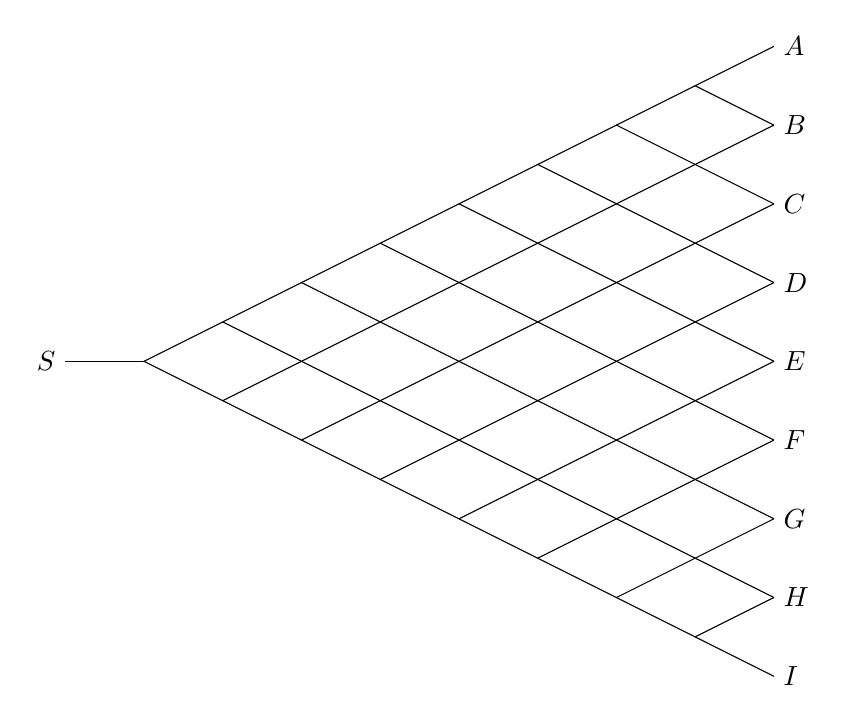
\begin{tikzpicture}
            \def\width{1}
            \def\height{0.5}
            \coordinate[label=left:$S$] (S) at (-1, 0);

            \coordinate (T0) at (0*\width, 0*\height);
            \coordinate (T1) at (1*\width, 1*\height);
            \coordinate (T2) at (2*\width, 2*\height);
            \coordinate (T3) at (3*\width, 3*\height);
            \coordinate (T4) at (4*\width, 4*\height);
            \coordinate (T5) at (5*\width, 5*\height);
            \coordinate (T6) at (6*\width, 6*\height);
            \coordinate (T7) at (7*\width, 7*\height);

            \coordinate (B1) at (1*\width, -1*\height);
            \coordinate (B2) at (2*\width, -2*\height);
            \coordinate (B3) at (3*\width, -3*\height);
            \coordinate (B4) at (4*\width, -4*\height);
            \coordinate (B5) at (5*\width, -5*\height);
            \coordinate (B6) at (6*\width, -6*\height);
            \coordinate (B7) at (7*\width, -7*\height);

            \coordinate[label=right:$A$] (A) at (8*\width, 8*\height);
            \coordinate[label=right:$B$] (B) at (8*\width, 6*\height);
            \coordinate[label=right:$C$] (C) at (8*\width, 4*\height);
            \coordinate[label=right:$D$] (D) at (8*\width, 2*\height);
            \coordinate[label=right:$E$] (E) at (8*\width, 0*\height);
            \coordinate[label=right:$F$] (F) at (8*\width, -2*\height);
            \coordinate[label=right:$G$] (G) at (8*\width, -4*\height);
            \coordinate[label=right:$H$] (H) at (8*\width, -6*\height);
            \coordinate[label=right:$I$] (I) at (8*\width, -8*\height);

            \draw (S) -- (T0);
            \draw (T0) -- (I);
            \draw (T1) -- (H);
            \draw (T2) -- (G);
            \draw (T3) -- (F);
            \draw (T4) -- (E);
            \draw (T5) -- (D);
            \draw (T6) -- (C);
            \draw (T7) -- (B);
            \draw (T0) -- (A);

            \draw (B1) -- (B);
            \draw (B2) -- (C);
            \draw (B3) -- (D);
            \draw (B4) -- (E);
            \draw (B5) -- (F);
            \draw (B6) -- (G);
            \draw (B7) -- (H);
        \end{tikzpicture}
    \end{center}

    \begin{enumerate}
        \item Show that the probability that the bug finishes its journey at D is $56p^5 q^3$.
        \item Given that the probability that the bug finishes its journey at D is greater than the probability at any one of the other endpoints, find exactly the possible range of values of $p$.
    \end{enumerate}

    In another version of the game, the probability that, at each junction, the bug takes the left fork is $0.9p$, the probability that the bug takes the right fork is $0.9q$ and the probability that the bug is swallowed up by a `black hole' is $0.1$.

    \begin{enumerate}
        \setcounter{enumi}{2}
        \item Find the probability that, in this version of the game, the bug reaches one of the endpoints A--I, without being swallowed up by a black hole.
    \end{enumerate}
\end{problem}
\begin{solution}
    \begin{ppart}
        Relabel each endpoint from A--I to 0--8. Let the random variable $X$ be the end-point that the bug ends up at. Clearly, to reach endpoint $i$, the bug must take $i$ right forks and $8-i$ left forks. Hence, $X \sim \Binom{8}{q}$ and the probability that the bug reaches endpoint 3 (i.e. endpoint D) is \[\P{X = 3} = \binom{8}{3} q^3 (1-q)^{8-3} = 56p^5q^3.\]
    \end{ppart}
    \begin{ppart}
        Since $X$ follows a binomial distribution, it suffices to find the range of values of $p$ that satisfy $\P{X = 2} < \P{X = 3} > \P{X = 4}$.
        
        \case{1}[$\P{X = 2} < \P{X = 3}$] Note that $\P(X = 2) = \binom{8}{2} q^2 (1-q)^{8-2} = 28p^6q^2$. \[\P(X = 2) < \P(X = 3) \implies 28p^6q^2 < 56p^5q^3 \implies 28p < 56(1-p) \implies p < \frac23.\]

        \case{2}[$\P{X = 3} > \P{X = 4}$] Note that $\P{X = 4} = \binom{8}{4} q^4 (1 - q)^{8-4} = 70 p^4 q^4$. \[\P(X = 3) > \P(X = 4) \implies 56p^5q^3 > 70p^4q^4 \implies 56p > 70(1-p) \implies p > \frac59.\]

        Hence, $5/9 < p < 2/3$.
    \end{ppart}
    \begin{ppart}
        Note that the bug most take a total of 8 forks. Since the probability of not getting swallowed by a black hole at each fork is $0.9$, the desired probability is clearly $0.9^8 = 0.430 \tosf{3}$.
    \end{ppart}
\end{solution}

\begin{problem}
    The number of injuries, $X$, sustained by workers in a factory per week follows a Poisson distribution with standard deviation $\s$. Given that $3\P{X = 2} = 16\P{X = 4}$ determine the value of $\s$ and hence state the mean of $X$.
    \begin{enumerate}
        \item Find the probability that, in a randomly chosen week, there is at least one injury.
        \item Assuming that a month consists of four weeks, find the probability that, in a randomly chosen month, there are less than 4 injuries.
        \item Calculate the probability that there will be more than 1 but less than 4 injuries in each of two consecutive weeks.
    \end{enumerate}
\end{problem}
\begin{solution}
    We have \[3\e^{-\m} \frac{\m^2}{2!} = 3\P{X = 2} = 16\P{X = 4} = 16\e^{-\m} \frac{\m^4}{4!} \implies \m^2 = \s = 2.25 \implies \m = 1.5.\] Thus, $X \sim \Po{1.5}$.
    \begin{ppart}
        $\P{X \geq 1} = 1 - \P{X = 0} = 0.777$.
    \end{ppart}
    \begin{ppart}
        Let $Y$ be the number of injuries in a month. Then $Y \sim \Po{6}$. Hence, $\P{Y < 4} = \P{Y \leq 3} = 0.151$.
    \end{ppart}
    \begin{ppart}
        The required probability is given by \[\bs{\P{1 < X < 4}}^2 = \bs{\P{X = 2} + \P{X = 3}}^2 = 0.142.\]
    \end{ppart}
\end{solution}

\begin{problem}
    During a weekday, heavy lorries pass a census point $P$ on a village high street independently and at random times. The mean rate for westward travelling lorries is 2 in any 30-minute period and for eastward travelling lorries is 3 in any 30-min period. Find the probability

    \begin{enumerate}
        \item that there will be no lorries passing $P$ in a given 10-min period,
        \item that at least one lorry from each direction will pass $P$ in a given 10-minute period,
        \item more than 2 westward travelling lorries will pass $P$ between the time 1410 and 1445,
        \item that there will be exactly 4 lorries passing $P$ in a given 20-minutes period
        \item at least 2 eastward travelling lorries passing $P$ in a period of 20 minutes given that there are exactly 4 lorries passing P at that time.
    \end{enumerate}
\end{problem}
\begin{solution}
    Let $W_k$ and $E_k$ be the number of westward and eastward travelling lorries passing $P$ in a $k$-minute period. Then \[W_k \sim \Po{\frac{k}{15}} \quad \land \quad E_k \sim \Po{\frac{k}{10}}.\]
    \begin{ppart}
        $\P{W_{10} = 0} \P{E_{10} = 0} = 0.189$.
    \end{ppart}
    \begin{ppart}
        $\P{W_{10} \geq 1} \P{E_{10} \geq 1} = \bs{1 - \P{W_{10} = 0}} \bs{1 - \P{E_{10} = 0}} = 0.308$.
    \end{ppart}
    \begin{ppart}
        $\P{W_{35} \geq 2} = 1 - \P{W_{35} \leq 2} = 0.413$.
    \end{ppart}
    \begin{ppart}
        Note that $W_{20} + E_{20} \sim \P{\frac{20}{15} + \frac{20}{10}} = \P{\frac{10}{3}}$. Thus, $\P{W_{20} + E_{20} = 4} = 0.184$.
    \end{ppart}
    \begin{ppart}
        The desired probability is given by \[1 - \frac{\P{W_{20} = 4}\P{E_{20} = 0} + \P{W_{20} = 3}\P{E_{20} = 1}}{\P{W_{20} + E_{20} = 4}} = 0.821.\]
    \end{ppart}
\end{solution}

\begin{problem}
    A car rental company has $n$ cars which may be hired on a daily basis. The demand for cars in a day follows a Poisson distribution with variance $1.5$. 
    \begin{enumerate}
        \item For $n=5$, for any one day,
        \begin{enumerate}
            \item find the probability that less than 3 cars are hired.
            \item find the probability that all the cars are hired.
        \end{enumerate}
        \item The probability that the demand for cars being met on any day is at least $0.95$. Find the least value of $n$.
        \item The probability that no car is rented out on $k$ consecutive days is less than $0.01$. Find the least value of $k$.
        \item The probability that there are less than two cars rented out on $h$ consecutive days is less than $0.005$. Find the least value of $h$.
    \end{enumerate}
\end{problem}
\begin{solution}
    Let $X$ be the number of cars hired in a given day. Then $X \sim \Po{1.5}$.
    \begin{ppart}
        \begin{psubpart}
            $\P{X < 3} = \P{X \leq 2} = 0.809 \tosf{3}$.
        \end{psubpart}
        \begin{psubpart}
            $\P{X \geq 5} = 1 - \P{X \leq 4} = 0.0186$.
        \end{psubpart}
    \end{ppart}
    \begin{ppart}
        Consider $\P{X \leq n} \geq 0.95$. Using G.C., the least $n$ is 4.
    \end{ppart}
    \begin{ppart}
        Consider $\P{X = 0}^k \leq 0.01$. Using G.C., the least $k$ is 4.
    \end{ppart}
    \begin{ppart}
        Consider $\P{X < 2}^h = \P{X \leq 1}^h \leq 0.005$. Using G.C., the least $h$ is 10.
    \end{ppart}
\end{solution}

\begin{problem}
    A randomly chosen doctor in general practices sees, on average, one case of a broken nose per year and each case is independent of other similar cases.

    \begin{enumerate}
        \item Regarding a month as a twelfth part of a year,
        \begin{enumerate}
            \item show that the probability that, between them, three such doctors see no cases of a broken nose in a period of one month is $0.779$, correct to three significant figures,
            \item find the variance of the number of cases seen by three such doctors in a period of six months.
        \end{enumerate}
        \item Find the probability that, between them, three such doctors see at least three cases in one year.
        \item Find the probability that, of three such doctors, one sees three cases and the other two see no cases in one year.
    \end{enumerate}
\end{problem}
\begin{solution}
    Let $X_{t,n}$ be the number of cases of a broken nose seen by $n$ doctors in $t$ months. Then $X \sim \Po{tn/12}$.
    \begin{ppart}
        \begin{psubpart}
            The required probability is \[\P{X_{1,3} = 0} = 0.779 \tosf{3}.\]
        \end{psubpart}
        \begin{psubpart}
            Since $X_{t,n}$ follows a Poisson distribution, $\m = \s^2$. Hence, \[\Var{X_{6, 3}} = \frac{(6)(3)}{12} = \frac32.\]
        \end{psubpart}
    \end{ppart}
    \begin{ppart}
        The required probability is \[\P{X_{12,3} \geq 3} = 1- \P{X_{12,3} \leq 2} = 0.577 \tosf{3}.\]
    \end{ppart}
    \begin{ppart}
        The required probability is \[\comb{3}{1} \P{X_{12,1} = 3}\P{X_{12,2} = 0} = 0.0249 \tosf{3}.\]
    \end{ppart}
\end{solution}

\begin{problem}
    During the winter in New York, the probability that snow will fall on any given day is $0.1$. Taking November 1st as the first day of winter and assuming independence from day to day, find the probability that the first snow of winter will fall in New York on the last day of November (30th).

    Given that no snow has fallen at New York during the whole of November, a teacher decides not to wait any longer to book a skiing holiday. The teacher decides to book for the earliest date for which the probability that snow will have fallen on, or before, that date is at least $0.9$. Find the date of the booking.
\end{problem}
\begin{solution}
    The probability that the first snow of winter will fall on 30 November is given by \[(0.9)^{29} (0.1) = 0.00471 \tosf{3}.\]

    Let $n$ be the number of days after 30 November. Consider $\P{X \leq n} \geq 0.9$, where $X \sim \Geo{0.1}$. Using G.C., the least $n$ is 22. Hence, the date of the booking is 22 December.
\end{solution}

\begin{problem}
    A salesman sells goods by telephone. The probability that any particular call achieves a sale is $1/12$. The salesman continues to make calls until one call achieves a sale.

    \begin{enumerate}
        \item State one assumption need for this to be modelled by a Geometric distribution.
        \item Given that a Geometric distribution is used to model this, find the probability that the call achieves a sale
        \begin{enumerate}
            \item is the fifth call made,
            \item does not occur in the first five calls.
        \end{enumerate}
        \item The salesman uses 5 minutes for each call, find the expected amount of time he has to spend to reach his first sale.
    \end{enumerate}
\end{problem}
\begin{solution}
    \begin{ppart}
        The calls must be independent.
    \end{ppart}
    \begin{ppart}
        Let $X$ be the number of calls made under the salesman achieves a sale. Then $X \sim \Geo{1/12}$.
        \begin{psubpart}
            $\P{X = 5} = 0.0588 \tosf{3}$.
        \end{psubpart}
        \begin{psubpart}
            $\P{X > 5} = (1 - 1/12)^5 = 0.647$.
        \end{psubpart}
    \end{ppart}
    \begin{ppart}
        Note that $\E{X} = 1/p = 12$. Hence, the expected amount of time he has to spend to reach his first sale is $5 \times 12 = 60$ minutes.
    \end{ppart}
\end{solution}

\begin{problem}
    If $X \sim \Binom{n}{p}$ and $Y \sim \Geo{p}$, explain why $\P{Y = n} \leq \P{X = 1}$.
\end{problem}
\begin{solution}
    Both $X = 1$ and $Y = n$ represent the event that there is exactly one success in $n$ trials. However, the event $Y = n$ has the added restriction that the success must come on the last trial, whereas the event $X = 1$ has no such restriction; the success can occur in any of the $n$ trials. Hence, the event $Y = n$ is a subset of the event $X = 1$, thus $\P{Y = n} \leq \P{X = 1}$, with equality only when $n = 1$.
\end{solution}

\begin{problem}
    Serious delays on a certain railway line occurs at random, at an average rate of one per week. Show that the probability of at least 4 serious delays occurring during a particular 4-week period is $0.567$, correct to 3 decimal places.

    Taking a year to consist of thirteen 4-week periods, find the probability that, in a particular year, there are at least ten of these 4-week periods during which at least 4 serious delays occur.

    Given that the probability of at least $n$ serious delays occurring in a period of 6 weeks is greater than $0.795$, find the largest possible integer value of $n$.
\end{problem}
\begin{solution}
    Let the number of serious delays in $k$ weeks be $X_k \sim \Po{k}$. We have \[\P{X_4 \geq 4} = 1 - \P{X_4 \leq 3} = 0.56653 = 0.567 \todp{3}.\]
    
    Let $Y$ be the number of 4-week periods during which at least 4 serious delays occur. Note that $Y \sim \Binom{13}{0.56653}$. Hence, \[\P{Y \geq 10} = 1 - \P{Y \leq 9} = 0.115 \tosf{3}.\]
    
    Consider $\P{X_6 \geq n} \geq 0.795$. Using G.C., the greatest value of $n$ is 4.
\end{solution}

\begin{problem}
    The demand for XO pies in a confectionary shop may be taken to follow a Poisson distribution with a mean of $0.4$ pies per hour. The shop opens for 5 days in a week and does business for 8 hours per day.

    \begin{enumerate}
        \item Find the probability that the demand for XO pies is at least 3 in a day.
        \item Find the probability that there is one day with demand for XO pies of at least 3, and another two days with demand 0.
        \item Find the probability that there is at most one day with zero demand for XO pies in a week.
        \item Given that the demand for XO pies is exactly 3 on a particular day, what is the probability that this occurred within the first hour of business.
    \end{enumerate}
\end{problem}
\begin{solution}
    Let the number of XO pies demanded in $k$ hours be $X_k \sim \Po{0.4k}$.

    \begin{ppart}
        $\P{X_8 \geq 3} = 1 - \P{X_8 \leq 2} = 0.620 \tosf{3}$.
    \end{ppart}
    \begin{ppart}
        Note that $\P{X_8 = 0} = 0.40762$. The required probability is \[\comb{3}{1} \P{X_8 \geq 3} \P{X_8 = 0} = 0.00309.\]
    \end{ppart}
    \begin{ppart}
        Let the number of days in a week where there is 0 demand for XO pies be $Y \sim \Binom{5}{0.40762}$. Then $\P{Y \leq 1} = 0.985 \tosf{3}$.
    \end{ppart}
    \begin{ppart}
        If all three pies for the day were sold within the first hour of business, then no pies were sold in the remaining seven hours. Hence, the required probability is \[\frac{\P{X_1 = 3}\P{X_1 = 0}^7}{\P{X_8 = 3}} = 0.00195.\]
    \end{ppart}

\end{solution}

\begin{problem}
    Given the climate of the country and duration of transportation, the probability of a strawberry from a particular orchard turning rotten is believed to be $0.15$. In a fruits wholesale centre where strawberries from that orchard are sold, they are packed and sold in trays of 20.

    \begin{enumerate}
        \item Show that the probability that there are at most 5 rotten strawberries in a tray is $0.933$.
        \item Find, to 3 decimal places, the probability that there are exactly 3 rotten strawberries in 2 randomly selected trays.
    \end{enumerate}
    
    A cold desserts hawker bought 60 trays of strawberries from the wholesaler centre. Using a suitable approximation, find the probability that there are at least 4 trays with more than 5 rotten strawberries in each tray.
\end{problem}
\begin{solution}
    Let $X_k$ be the number of rotten strawberries in $k$ trays. We have $X_k \sim \Binom{20k}{0.15}$.
    \begin{ppart}
        $\P{X_1 \leq 5} = 0.933 \tosf{3}$.
    \end{ppart}
    \begin{ppart}
        $\P{X_2 = 3} = 0.0816 \tosf{3}$.
    \end{ppart}

    Note that $\P{X_1 > 5} = 1 - \P{X_1 \leq 5} = 0.067308$. Let $Y$ be the number of trays with more than 5 rotten strawberries. We can approximate $Y$ using a Poisson distribution since $n = 60$ is large and $p = 0.067308$ is small. We hence have $Y \sim \Po{np} = \Po{4.0385}$. Then $\P{Y \geq 4} = 1 - \P{Y \leq 3} = 0.574 \tosf{3}$.
\end{solution}